% !TEX TS-program = xelatex
% !TEX encoding = UTF-8 Unicode

\documentclass[11pt,a4paper,english]{article} % document type and language

% Laad stijlen via relatieve paden
\newcommand{\path}{C:/Users/Admin/Documents/GitHub/Statistiek}
\usepackage{\path/LaTeX/styles/config}
\usepackage{\path/LaTeX/styles/statistics-macros}
\graphicspath{{\path/LaTeX/figures/}}

\usetikzlibrary{shapes.geometric, arrows.meta, positioning}
\setlength{\parindent}{0cm} 

\tikzstyle{startstop} = [rectangle, rounded corners, minimum width=3cm, minimum height=1cm, rounded corners, text centered, draw=black, fill=blue!20]
\tikzstyle{decision} = [rectangle, minimum width=3cm, minimum height=1cm, rounded corners, text centered, draw=black, fill=orange!30]
\tikzstyle{process} = [rectangle, minimum width=3.5cm, minimum height=1cm, rounded corners, text centered, draw=black, fill=green!20]
\tikzstyle{arrow} = [thick,->,>=stealth]

\begin{document}
\section*{Formula sheet - Probability \& Statistics (PMTPS)}

\textbf{Law of total probability:}
\[ P(B) = P(B|A)P(A) + P(B|A')P(A')\]

\textbf{Bayes' Rule:}
\[ P(A|B) = P(B|A) \cdot \frac{P(A)}{P(B)} \]

\textbf{Expected value:}
\[
    E(X) = \sum_{x} x \cdot P(X = x) \qquad (\text{discrete})
\]
\[
    E(X) = \int_{x} x \cdot f(x)\ dx \qquad (\text{continuous})
\]

\textbf{Sample mean:}
\[
    \overline{x} = \frac{\sum_{i=1}^{n} x_{i}}{n}
\]

\textbf{Variance:}
\[
    \Var{X} = \sum_{x} \left(x - E(X)\right)^2 \cdot P(X = x) = E(X^2) - E(X)^2 \qquad (\text{discrete})
\]
\[
    \Var{X} = \int_{x} \left(x-E(X)\right)^2 \cdot f(x)\ dx = E(X^2) - E(X)^2 \qquad (\text{continuous})
\]

\textbf{Sample variance:}
\[
    s^2 = \frac{1}{n-1}\sum_{i=1}^{n} (x_{i} - \overline{x})^2
\]

\textbf{Covariance:}
\[
    \Cov{X}{Y} = E\left((X-E(X))\cdot(Y-E(Y))\right) = E(X \cdot Y) - E(X)E(Y)
\]

\textbf{Correlation coefficient:}
\[
    \rho(X, Y) = \frac{\Cov{X}{Y}}{\sigma(X) \cdot \sigma(Y)}
\]

\textbf{Variance of error terms:}
\[ \hat{\sigma}^2 = \frac{1}{n-2}\sum_{i=1}^{n} (y_{i} - \hat{y}_{i})^2 = \frac{\sum_{i=1}^{n} y_{i}^2 - \hat{\beta}_{0}\cdot \sum_{i=1}^{n} y_{i} - \hat{\beta}_{1}\cdot \sum_{i=1}^{n} x_{i}y_{i}}{n-2}\]

\textbf{Coefficients of regression line:}

Given a sample of $n$ observations $(x_1, y_1), (x_2, y_2), \ldots, (x_n, y_n)$, the regression line $\hat{y} = \hat{\beta}_0 + \hat{\beta}_{1}\cdot x$ satisfies:
\begin{itemize}
    \item $\hat{\beta}_{1} = \frac{\sum_{i=1}^{n}x_iy_i - n \cdot \overline{x} \cdot \overline{y}}{\sum_{i=1}^{n} x_{i}^2 - n \cdot \overline{x}^2} = \frac{\overline{xy}-\overline{x}\cdot \overline{y}}{\overline{x^2}-\overline{x}^2}$
    \item $\hat{\beta}_{0} = \overline{y} - \hat{\beta}_{1} \cdot \overline{x}$
\end{itemize}

\textbf{Sample correlation coefficient:}
\[ r(x, y) = \frac{\Cov{x}{y}}{\sqrt{s_{X}^2\cdot s_{Y}^2}} = \frac{\overline{xy} - \overline{x} \cdot \overline{y}}{\sqrt{(\overline{x^2} - \overline{x}^2)\cdot(\overline{y^2} - \overline{y}^2)}}\]

\textbf{Likelihood function:}
\[ L(x_1, x_2, \ldots, x_n; \theta) = \prod_{i=1}^n f(x_i; \theta) = f(x_1; \theta)\cdot f(x_2; \theta)\cdot\ldots\cdot f(x_n; \theta)\]

\textbf{Minimum sample size with given accuracy $E$:}
\[ n \ge \left(\frac{z_{\alpha/2} \cdot \sigma}{E}\right)^2\]

\textbf{Minimum sample size for bounding type II error $\beta$}
\[ n \ge \frac{(z_{\alpha/2}+z_{\beta})^2 \cdot \sigma^2}{\delta^2}\]

\textbf{Expected values and variance of common probability distributions:}
\begin{table}[h!]
\centering
\begin{tabular}{cp{5cm}ccc}
\toprule
\textbf{Distribution} & \textbf{PMF/PDF} & \textbf{CDF} & \textbf{Mean} & \textbf{Variance} \\ \midrule
\multicolumn{5}{c}{\textbf{Discrete}} \\ \midrule
Uniform($a, b$) & $P(X=k) = \frac{1}{b-a+1}$ \newline $(k=a,a+1,\ldots,b)$ & $F(k) = \begin{cases} 
0 & x < a \\
\frac{k - a + 1}{b-a+1} & a \leq k < b \\
1 & k \geq b
\end{cases}$ & $\frac{a+b}{2}$ & $\frac{(b-a+1)^2-1}{12}$ \\ \midrule
Bernoulli($p$) & $P(X=k) = \begin{cases} 1-p, & \text{$k=0$} \\ p, & \text{$k=1$} \end{cases}$ & $F(k) = \begin{cases} 
0 & k < 0 \\
1-p & k=0 \\
1 & k \geq 1
\end{cases}$ & $p$ & $p(1-p)$ \\ \midrule
Binomial($n,p$) & $P(X=k) = \binom{n}{k}p^k(1-p)^{n-k}$ & $F(k) = \sum_{i=0}^k \binom{n}{i}p^i(1-p)^{n-i}$ & $np$ & $np(1-p)$ \\ \midrule
Geometric($p$) & $P(X=k) = (1-p)^{k-1}\cdot p$ & $F(k) = \sum_{i=1}^k(1-p)^{k-1}\cdot p$ & $\frac{1}{p}$ & $\frac{1-p}{p^2}$ \\ \midrule
Poisson($\lambda$) & $P(X=k) = e^{-\lambda}\cdot \frac{\lambda^k}{k!}$ & $F(k) = \sum_{i=0}^k \frac{\lambda^i e^{-\lambda}}{i!}$ & $\lambda$ & $\lambda$ \\ \midrule
\multicolumn{5}{c}{\textbf{Continuous}} \\ \midrule
Uniform($a, b$) & $f(x) = \begin{cases} \frac{1}{b-a}, & a \leq x \leq b \\ 0, & \text{otherwise.} \end{cases}$ & $F(x) = \begin{cases} 
0, & x < a \\
\frac{x-a}{b-a}, & a \leq x < b \\ 1, & x \geq b \end{cases}$ & $\frac{a+b}{2}$ & $\frac{(b-a)^2}{12}$ \\ \midrule
Normal($\mu, \sigma^2$) & $f(x) = \frac{1}{\sigma\cdot\sqrt{2\pi}} e^{-\frac{1}{2}\left(\frac{x-\mu}{\sigma}\right)^2}$ & $\Phi\left(\frac{x-\mu}{\sigma}\right)$ & $\mu$ & $\sigma^2$ \\ \midrule
Exponential($\lambda$) & $f(x) = \lambda e^{-\lambda x}$, $x \geq 0$ & $F(x) = \begin{cases} 1 - e^{-\lambda x}, & x \geq 0 \\ 0, & x < 0 \end{cases}$ & $\frac{1}{\lambda}$ & $\frac{1}{\lambda^2}$ \\ 
\bottomrule
\end{tabular}
% \caption{Discrete and Continuous Probability Distributions with Mean and Variance}
% \label{tab:prob_dist}
\end{table}

\newpage

\textbf{Types of hypothesis tests}
\begin{table}[H]
    \centering
    \renewcommand{\arraystretch}{1.5}
    \begin{tabular}{m{0.2\textwidth}m{0.25\textwidth}m{0.40\textwidth}}
        \toprule
            \textbf{Test name} & \textbf{Test statistic} & \textbf{Probability distribution (under $H_0$)} \\
        \midrule
            \multicolumn{3}{c}{\textbf{Tests for the mean $\mu$ of a normal distribution}} \\ 
        \midrule
            $\sigma$ known    & $\overline{X}$ & $N(\mu_0, \sigma / \sqrt{n})$ \\
            $\sigma$ unknown  & $T = \frac{\overline{X} - \mu_0}{S / \sqrt{n}}$ & $t(\df=n-1)$ \\
        \midrule
            \multicolumn{3}{c}{\textbf{Chi-square test ($\chi^2$)}} \\
        \midrule
            Chi-square \newline goodness-of-fit & $X^2 = \sum_{i} \frac{(O_{i} - E_{i})^2}{E_{i}}$ & $\chi^2\left(\df=\text{\#categories-1}\right)$ \\
        % \midrule
        %     \multicolumn{4}{c}{\textbf{Toetsen op basis van twee onafhankelijke populaties $A$ en $B$ (met steekproefgroottes $n$ en $m$)}} \\
        % \midrule
        %     $F$-toets & $\sigma_A^2 = \sigma_B^2$ & $F = \frac{S_A^2}{S_B^2}$ & $F\left(\df_A = n-1, \df_B = m-1\right)$ \\
        %     $z$-toets & $\mu_A \leq/=/\geq \mu_B$ & $Z = \frac{(\overline{X_A} - \overline{X_B}) - (\mu_A - \mu_B)}{\sqrt{\frac{\sigma_A^2}{n} + \frac{\sigma_B^2}{m}}}$ & $N\left(\mu=0, \sigma=1\right)$ \\
        %     $t$-toets ($\sigma_A^2 = \sigma_B^2$) & $\mu_A \leq/=/\geq \mu_B$ & $T = \frac{(\overline{X_A} - \overline{X_B}) - (\mu_A - \mu_B)}{\sqrt{\frac{S_P^2}{n} + \frac{S_P^2}{m}}}$ & $t\left(\df=n+m-2\right)$ \\
        %     $t$-toets ($\sigma_A^2 \neq \sigma_B^2$) & $\mu_A \leq/=/\geq \mu_B$ & $T = \frac{(\overline{X_A} - \overline{X_B}) - (\mu_A - \mu_B)}{\sqrt{\frac{S_A^2}{n} + \frac{S_B^2}{m}}}$ & $t\left(\df=\min(n-1, m-1)\right)$ \\
        \bottomrule
    \end{tabular}
\end{table}

\textbf{One-sided and two-sided hypothesis tests}

\begin{tabular}{@{}c@{}c@{}c@{}}
    \textbf{Left-sided} & \textbf{Two-sided} & \textbf{Right-sided} \\
    $H_0: \mu \geq \mu_0 \text{ vs. } H_1: \mu < \mu_0$ & $H_0: \mu = \mu_0 \text{ vs. } H_1: \mu \neq \mu_0$ & $H_0: \mu \leq \mu_0 \text{ vs. } H_1: \mu > \mu_0$ \\
    Acceptance region: {\color{green!50!black} $[g, \infty)$} & Acceptance region: {\color{green!50!black} $[g_1, g_2]$} & Acceptance region: {\color{green!50!black} $(-\infty, g]$} \\
    Critical region: {\color{red} $(-\infty, g)$} & Critical region: {\color{red} $(-\infty, g_1)$ and $(g_2, \infty)$} & Critical region: {\color{red} $(g, \infty)$} \\
    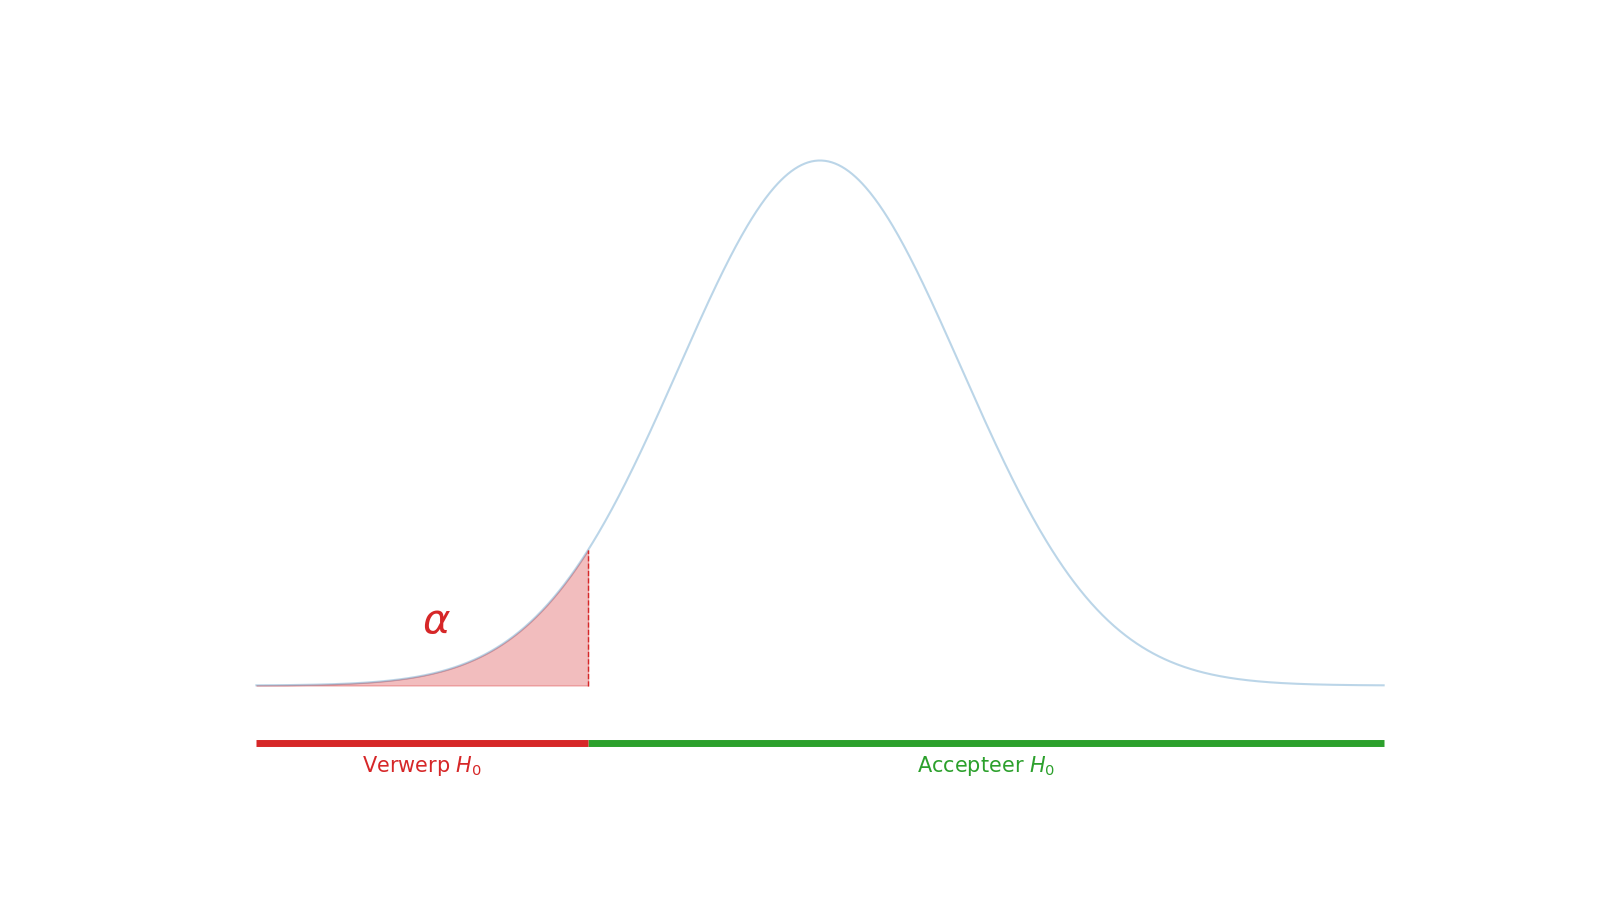
\includegraphics[width=0.33\textwidth]{../../LaTeX/figures/linkszijdig.png} & 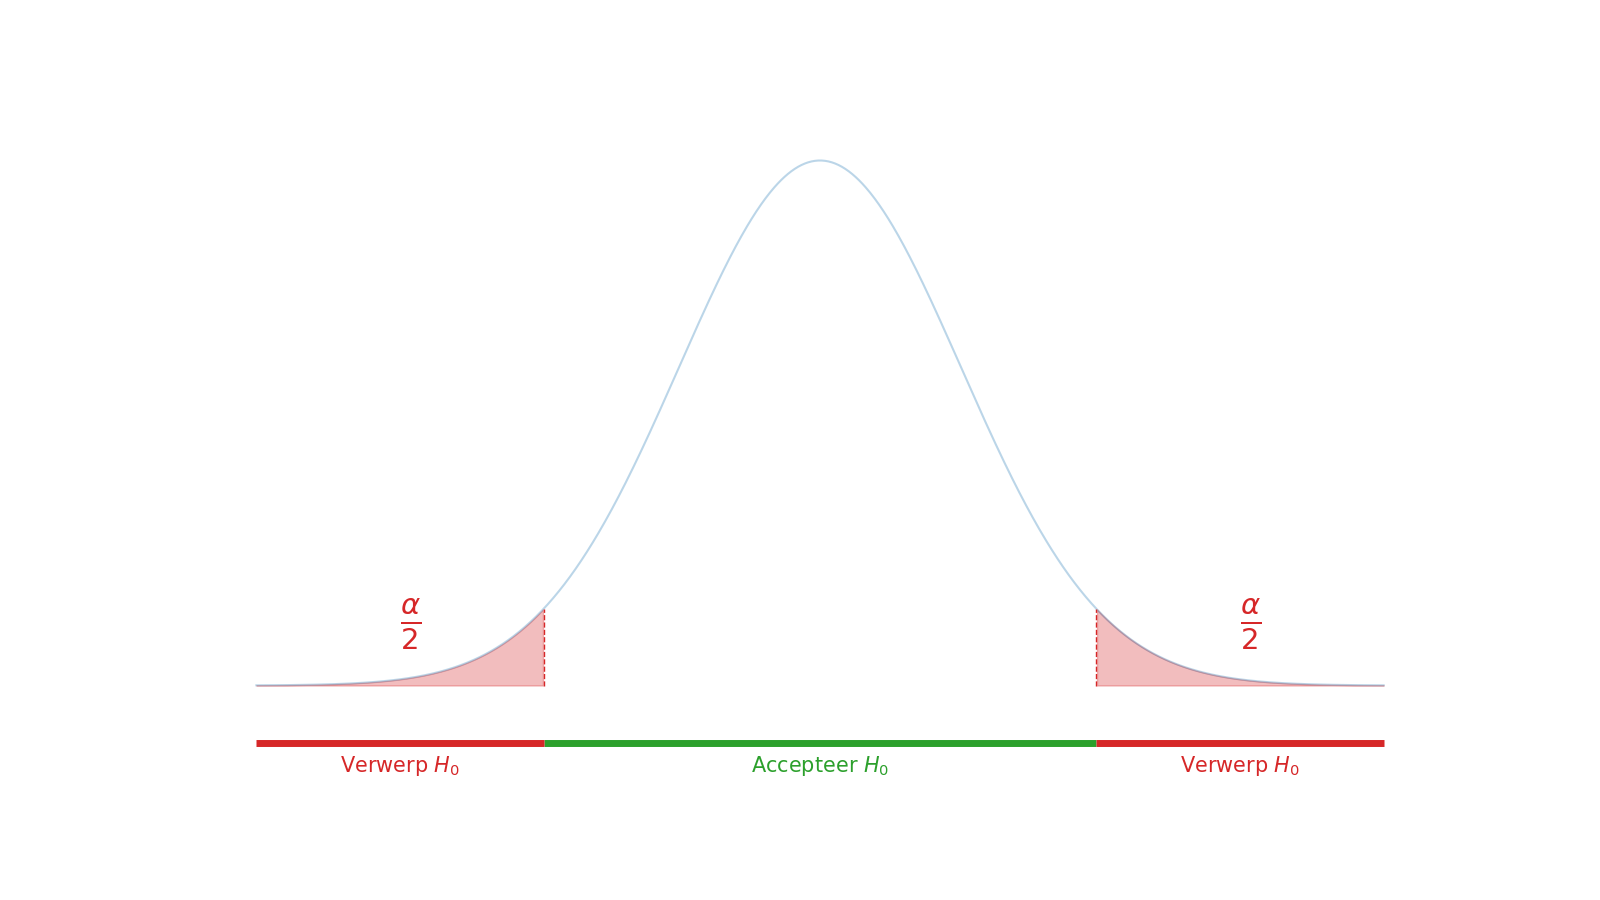
\includegraphics[width=0.33\textwidth]{../../LaTeX/figures/tweezijdig.png} & 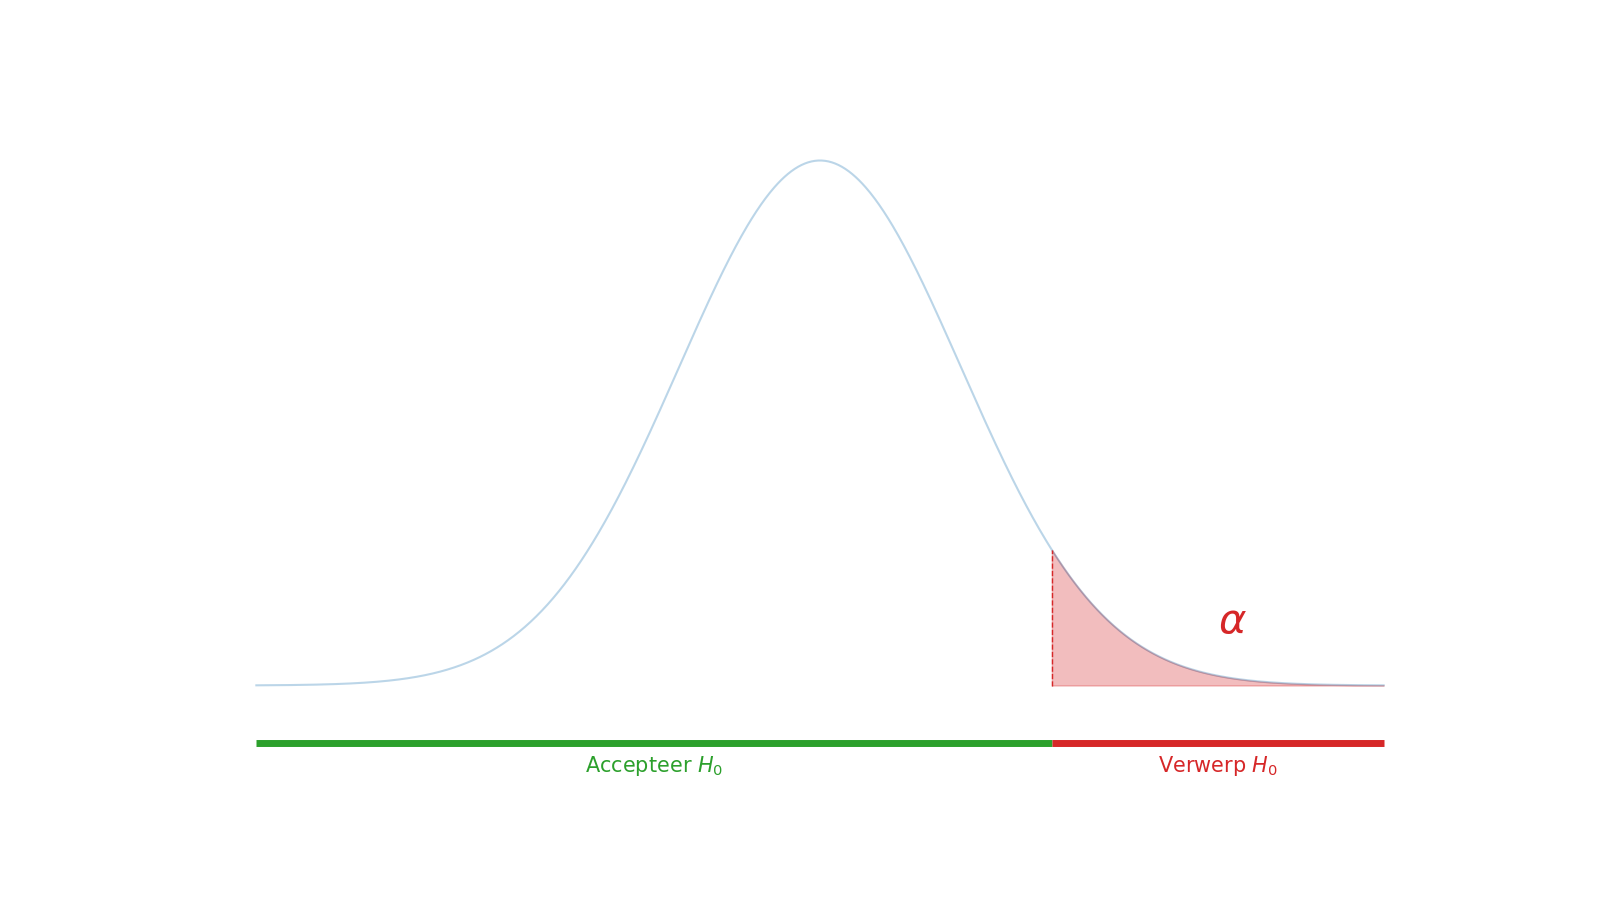
\includegraphics[width=0.33\textwidth]{../../LaTeX/figures/rechtszijdig.png}\\
\end{tabular}

\textbf{Critical regions}
\begin{table}[H]
    \centering
    \renewcommand{\arraystretch}{1.5}
    \begin{tabular}{m{2.5cm}|m{4cm}|m{5cm}|m{4cm}}
        \toprule
            \textbf{Probability distribution (under $H_0$)} & \textbf{Left-sided} \newline $(-\infty, g)$ & \textbf{Two-sided} \newline $(-\infty, g_1)$ and $(g_2, \infty)$ & \textbf{Right-sided} \newline $(g, \infty)$ \\
        \midrule
            \multirow{2}*{$N\left(\mu, \sigma\right)$} & \multirow{2}*{$g = \invnorm(\alpha, \mu, \sigma)$} & $g_1 = \invnorm(\alpha / 2, \mu, \sigma)$ & \multirow{2}*{$g = \invnorm(1-\alpha, \mu, \sigma)$}\\
            & & $g_2 = \invnorm(1-\alpha / 2, \mu, \sigma)$ & \\
        \midrule
            \multirow{2}*{$t(\df)$} & \multirow{2}*{$g = \invt(\alpha, \df)$} & $g_1 = \invt(\alpha / 2, \df)$ & \multirow{2}*{$g = \invt(1-\alpha, \df)$}\\
            & & $g_2 = \invt(1-\alpha / 2, \df)$ & \\
        \midrule
            \multicolumn{4}{c}{\emph{Boundary values that need to be solved with the \enquote{numeric solver}:}} \\
        \midrule
            $\chi^2(\df)$ & - & - & $\chi^2\text{cdf}(g, 10^{99}, \df) = \alpha$\\
        \bottomrule
    \end{tabular}
\end{table}

\newpage

\textbf{$p$-values (for given theoretical and observed test statistics $T$ and $t$)}

    \begin{table}[H]
        \centering
        \renewcommand{\arraystretch}{1.5}
        \begin{tabular}{m{4.5cm}|cc}
            \toprule
                \textbf{Probability distribution (under $H_0$)} & \textbf{Left-sided test: $P(T \le t)$} & \textbf{Right-sided test: $P(T \ge t)$} \\
            \midrule
                $N(\mu, \sigma)$ & $p = \normalcdf(-10^{99}, t, \mu, \sigma)$ & $p = \normalcdf(t, 10^{99}, \mu, \sigma)$ \\
            \midrule
                $t(\df)$ & $p = \tcdf(-10^{99}, t, \df)$ & $p = \tcdf(t, 10^{99}, \df)$\\
            \midrule
                $\chi^2(\df)$ & - & $p = \chi^2\text{cdf}(t, 10^{99}, \df)$ \\
            \bottomrule
        \end{tabular}
    \end{table}

    {\itshape Note: with two-sided tests, the $p$-value is equal to the minimum of $P(T \leq t)$ and $P(T \geq t)$.}
\vspace{0.5cm}

\end{document}
